\chapter{Impresión del horario en PDF}

\section{Introducción}
Hemos implementado una función capaz de transformar la matriz 3D en la que almacenamos nuestros horarios en un documento \LaTeX. El objetivo de esto es conseguir un resultado lo más parecido posible a las tablas actuales de horarios, que se realizan a mano. En la \hyperref[horario_actual]{Imagen \ref*{horario_actual}} se ve una de las tablas que se usan actualmente y en la \hyperref[horario_implementado]{Figura \ref*{horario_implementado}} se ve la implementación en \LaTeX\; realizada. La estructura es prácticamente idéntica, la única diferencia entre ambas es que la tabla implementada no es tan alargada como la de la facultad y que la leyenda de nombres de cada asignatura se encuentra justo debajo de la tabla en lugar de al lado.

\begin{figure}[H]
    \centering
    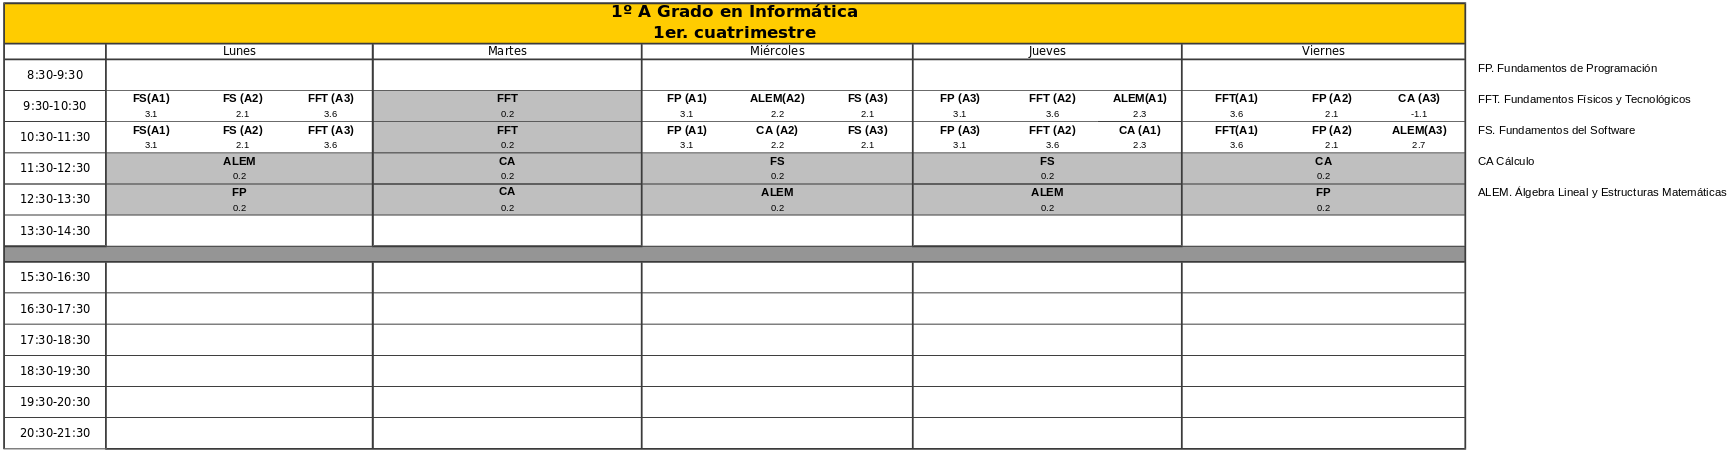
\includegraphics[width=\textwidth]{img/horario_actual}
    \label{horario_actual}
    \caption{Estructura actual del PDF de horarios.}
\end{figure}

\begin{figure}[H]
    \centering
    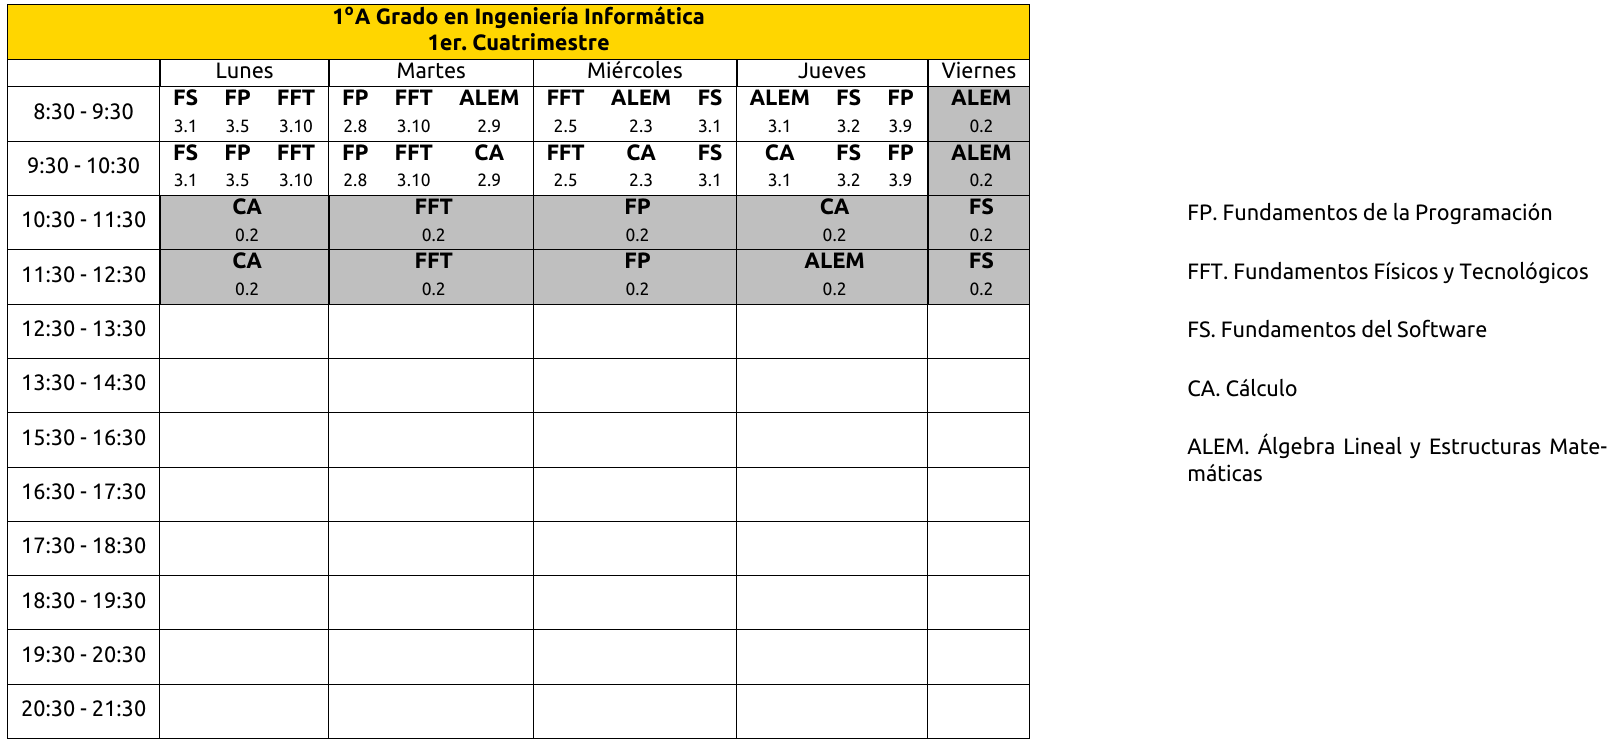
\includegraphics[width=\textwidth]{img/horario_implementado}
    \label{horario_implementado}
    \caption{Estructura implementada del PDF de horarios.}
\end{figure}

\section{Sobre la tabla \LaTeX}
En primer lugar, hemos definido una cabecera \LaTeX\; sencilla, en la que eliminamos las cabeceras por defecto de \LaTeX usando el paquete \texttt{fancyhdr}. Dicha cabecera, se lee justo al principio y se almacena en una variable como un \texttt{string}. Después, para cada grupo, se genera una tabla horario. Hay varias cosas a tener en cuenta a la hora de generar la tabla.

En \LaTeX\; no se puede dividir una celda en varias subceldas, sino que pueden unirse varias celdas en una sola. Esto hace que si hay tres subgrupos de prácticas en un grupo, su tabla de horarios tenga 16 columnas. Los días de la semana y las horas teóricas serán el resultado de unir tres celdas en una sola mientras que las celdas de prácticas, serán una única celda \LaTeX. Para unir celdas, se usa la instrucción \texttt{multicolumn} de \LaTeX.:

\begin{minted}[frame=lines, label={Cabecera de una tabla LaTeX y multicolumn}]{latex}
\begin{tabular}{|c|ccc|ccc|ccc|ccc|ccc|}
\hline
\rowcolor{amarillo} \multicolumn{16}{|c|}{\textbf{1ºA Grado ...}}\\ 
\rowcolor{amarillo} \multicolumn{16}{|c|}{\textbf{1er. Cuatrimestre}}\\ 
\hline 
 & \multicolumn{3}{|c|}{Lunes} & \multicolumn{3}{|c|}{Martes} & ... \\
\end{minted}

Al igual que pasa con las columnas, las filas tampoco se pueden dividir. Por eso, las horas del día ocupan dos filas distintas usando la instrucción \texttt{multirow}, después, se crea una fila con las asignaturas y otra fila con las aulas:

\begin{minted}[frame=lines, label={Multirow}]{latex}
\multirow{2}{*}{8:30 - 9:30}  & \textbf{FFT} & \textbf{FP} & \textbf{FS}...\\ 
 & {\footnotesize 2.5} & {\footnotesize 3.9} & {\footnotesize 2.1}...\\ 
 \hline
\end{minted}

Por último, para poder dividir en dos una página de \LaTeX, usamos el entorno \texttt{minipage}. Este entorno permite crear una ``mini-página'', que ocupa un determinado ancho (\texttt{textwidth}) de la página actual. Si ponemos dos \texttt{minipage} uno justo debajo del otro, se creará el efecto de dos columnas con la flexibilidad de poder ajustar el ancho de cada una de forma cómoda:

\begin{minted}[frame=lines, label={Ejemplo de uso de minipage}]{latex}
\begin{minipage}{0.7\textwidth}
...
\end{minipage}
\begin{minipage}{0.25\textwidth}
...
\end{minipage}
\end{minted}

